%------------------------------------------------
\section{Introducción} 
%------------------------------------------------

\subsection{Descripción}
 
%%%% IDEAS %%%%
% Modulable y expandible
% Color LEDs blanco
% Bloque de 8x7 minimo..
% Modular la velocidad
% Juego mario, dinosaurio chrome

%% DEFF CANTIDAD DE LETRAS POR RENGLON %%
\newcommand\cantLetrasRenglon{3}
%% ----------------------------------- %%

\begin{frame}
	\frametitle{Descripción}
	
		\begin{block}{Motivación}
			\begin{itemize}
				\item Alto costo de productos en el mercado
				\item Reducción del uso de papel
			\end{itemize}
		\end{block}

		\begin{block}{Características generales}
			\begin{itemize}
				\item Caracteres de 8x7 píxeles
				\item Módulos expansibles
				\item Control por WiFi
				\item Animación programable
			\end{itemize}
		\end{block}

\end{frame}

\subsection{Objetivos}
\begin{frame}
	\frametitle{Objetivos}
	\begin{block}{Objetivos primarios}
		\begin{itemize}
			\item Diseñar e implementar el Hardware (PCB, Cartel)
			\item Diseñar e implementar protocolo de comunicación
			\item Desarrollar el Software que se ejecutará en el microcontrolador
			\item Desarrollar el Software que controla el cartel
		\end{itemize}
	\end{block}
\end{frame}

%------------------------------------------------
\section{Especificación}
%------------------------------------------------

\subsection{Requerimientos}
\begin{frame}
	\frametitle{Requerimientos}
	\begin{block}{Funcionales}
		\begin{itemize}
			\item El cartel debe ser configurable a través de WiFi
			\item El contenido que muestre el cartel debe ser persistente
			\item El control del cartel debe requerir autenticación
		\end{itemize}
	\end{block}

	\begin{block}{No funcionales}
		\begin{itemize}
			\item El tiempo de desarrollo no debe ser mayor a seis semanas
			\item Debe usarse la EDU-CIAA
			\item La conexión debe estar cifrada
		\end{itemize}
	\end{block}

\end{frame}

\subsection{Diagrama en bloques del sistema}
\begin{frame}
	\frametitle{Diagrama en bloques}
	\begin{figure}[htbp]
		\begin{center}
			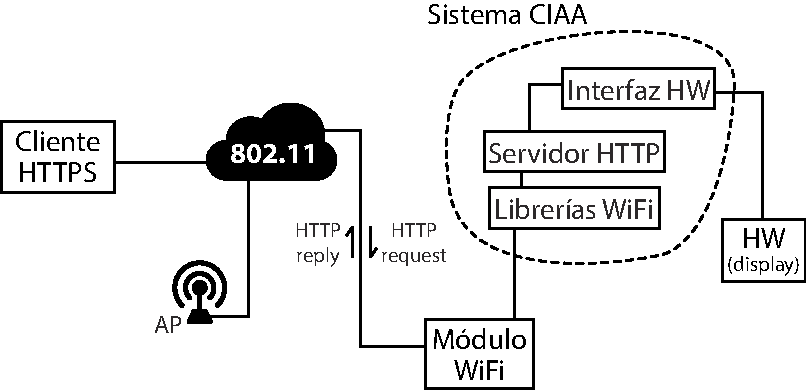
\includegraphics[width=\textwidth]{diagramas/diagrama-bloques.pdf}
			\caption{Esquema gráfico del sistema completo.}
			\label{fig:diagrama-bloques}
		\end{center}
	\end{figure}
\end{frame}

\subsection{Explicación funcional del HW y SW}
\begin{frame}
	\frametitle{Explicación funcional}
	\begin{itemize}
		 \item El sistema se conecta una red WiFi preexistente y escucha conexiones TLS
		 \item El usuario accede, autenticándose, al cartel utilizando una aplicación de escritorio
		 \item El usuario ingresa el anuncio a mostrar junto a los parámetros de animación (parpadeo y velocidad de desplazamiento)
		 \item El sistema interpreta la orden y controla el cartel como corresponda
	\end{itemize}
	
	% El microcontrolador que maneja el cartel compuesto de LED's, es el encargado de establecer una red WIFI (sin acceso a internet) sobre la cual hostea un panel de configuración. Por medio de un usuario y clave, se accede al panel vía https y se puede cambiar el anuncio a representar en el cartel. El mensaje a representar, se desplaza a lo largo de la matriz de LED's a modo de marquesina y, dentro del panel, se pueden configurar determinados parámetros como por ejemplo, la velocidad a la que se mueve.

\end{frame}

%------------------------------------------------
\section{Gestión}
%------------------------------------------------

\subsection{Presupuesto}
\begin{frame}
	\frametitle{Presupuesto}
	\FPeval{\cantLEDs}{round( 64*\cantLetrasRenglon , 0)}
	\FPeval{\cantChips}{round( 1*\cantLetrasRenglon , 0)}
	\begin{table}[]
		\centering
		\caption{Presupuesto tentativo. (Cantidades en ARS)}
		\begin{spreadtab}{{tabular}{cccc}}
			@ Item				& @ Unidades	& @ Precio unidad	& @ Subtotal	\\ \hline
			@ Componentes varios& :={} -		& :={} -			& 80  \\
			@ PCB				& \cantLEDs		& \$ :={30}			& b3*c3  \\
			@ LEDs				& \cantLEDs		& \$ :={1}			& b4*c4  \\
			@ Gabinete         	& 1				& \$ :={2000}		& b5*c5  \\
			@ ESP8266			& 1				& \$ :={200}		& b6*c6  \\
			@ EDU-CIAA			& 1				& \$ :={1000}		& b7*c7  \\
			@ MAX7219			& \cantChips	& \$ :={45}			& b8*c8	 \\
			@ Horas hombre		& :={20*5*3} hs	& \$ :={200}		& b9*c9  \\ \hline
			@ Total				& 				&					& sum(d2:d9)	 \\ \hline
		\end{spreadtab}
	\end{table}
\end{frame}


\subsection{Cronograma}
\begin{frame}
	\frametitle{Cronograma}
    \begin{figure}[htbp]
		\begin{center}
			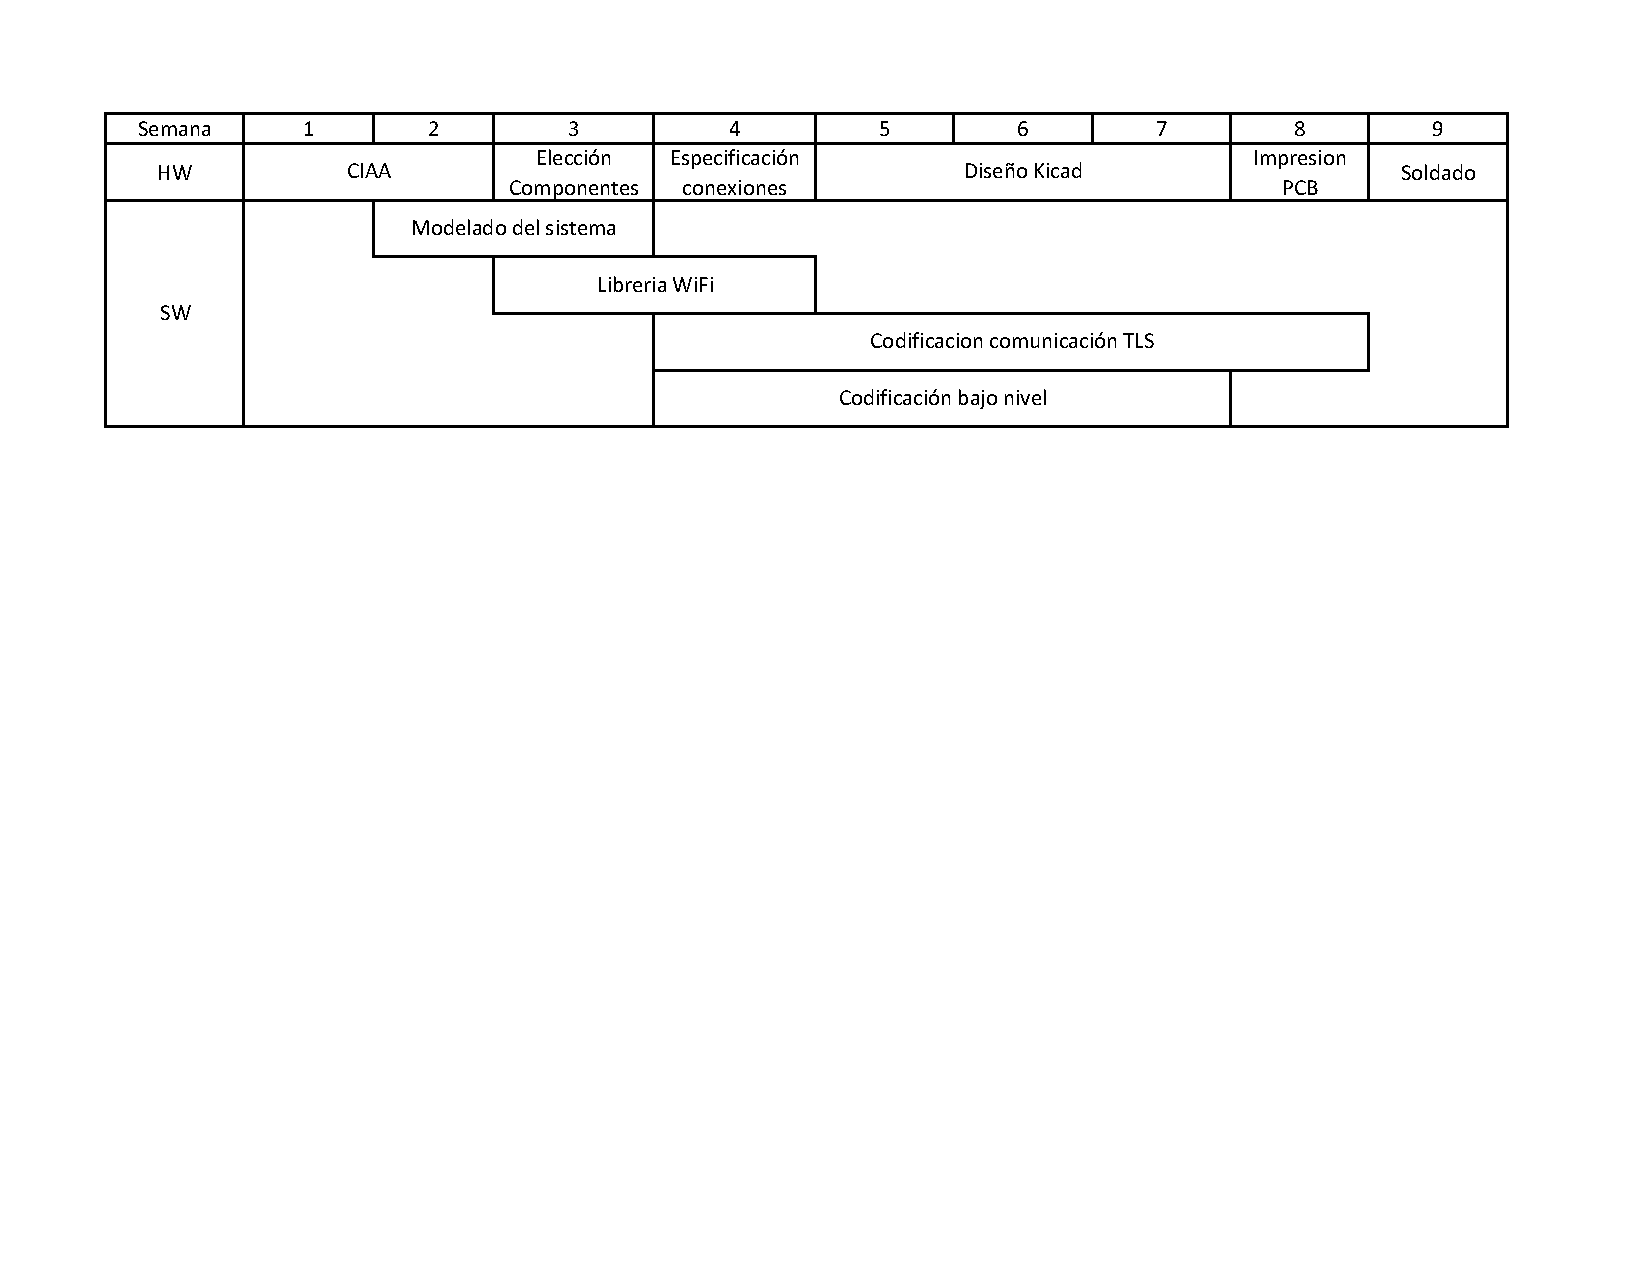
\includegraphics[width=\textwidth]{diagramas/cronograma.pdf}
			\caption{Asignación de tiempos aproximados.}
			\label{fig:diagrama-cronograma}
		\end{center}
	\end{figure}
\end{frame}

\subsection{División de tareas del grupo}
\begin{frame}
	\frametitle{División de tareas del grupo}
	\begin{itemize}
		\item \textbf{García}: Diseño del protocolo y desarrollo de software para ESP8266 y EDU-CIAA
		\item \textbf{Romero Dapozo}: Diseño del protocolo, desarrollo de Software para ESP8266 y aplicación de escritorio
		\item \textbf{Ternouski}: Diseño y armado del Hardware y aplicación de escritorio
		\item \textbf{Levy}: Diseño y armado del Hardware
	\end{itemize}
\end{frame}

%------------------------------------------------
\section{Referencias}
%------------------------------------------------
\iffalse
\begin{frame}
	\frametitle{Referencias}
	\footnotesize{
	\begin{thebibliography}{99}
		\bibitem[Nielsen, 2001]{ref:Nielsen} Nielsen, Jakob. (2001)
		\newblock Beyond Accessibility: Treating People with Disabilities as People.
		\newblock \emph{Alertbox}.
		Disponible en:
		\href{http://www.useit.com/alertbox/20011111.html}{www.useit.com}
	\end{thebibliography}
	}
\end{frame}
\fi